\newprob{1715330504}
{
支架$PQ$上架了一樑橫木,如圖。横木重 \qty{300}{N}。 有一個重 \qty{600}{N} 的人從$Q$點,慢慢向右走。
{\par\centering
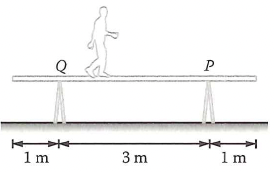
\includegraphics[width=.3\textwidth]{assets/efd30991.png}
\par}
那人走到何處,橫木就會翻起?
\begin{tasks}
    \task $P$點之右 \qty{0.5}{m}
    \task $P$點之左 \qty{0.5}{m}
    \task $P$點之右 \qty{0.75}{m}
    \task $P$點之左 \qty{0.75}{m}
\end{tasks}
}{C}

\newprob{1715331378}
{
如圖,一塊高 \qty{5}{cm} 、底長 \qty{12}{cm} 、且重量為 \qty{10}{N} 的三角木塊$ABC$放在水平面上。當一道量值 \qty{3}{N} 的施力$F$ 向左作用於 $A$ 點時,木塊開始翻側。現在如果 $F$ 指向右,其量值應為多少,方能使木塊開始翻側?
{\par\centering
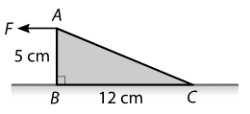
\includegraphics[width=.3\textwidth]{assets/ad661d08.png}
\par}
\begin{tasks}
    \task \qty{6.2}{N}
    \task \qty{8.1}{N}
    \task \qty{16}{N}
    \task \qty{21}{N}

\end{tasks}
}{D}

\newprob{1715331721}
{
一磚勻質方塊,高 $h$ 闊$\ell$,擱在地毯上。把地毯 以加速度 $a$ 水平拉動。

{\par\centering
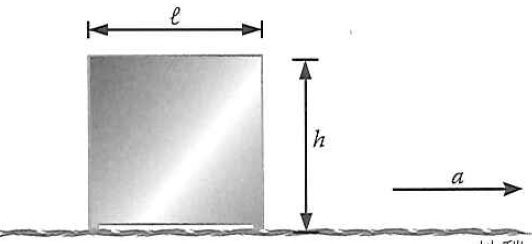
\includegraphics[width=.3\textwidth]{assets/5b765e46.png}
\par}
假設方塊沒有翻側,也沒有滑移,$a$ 的最大值是 多少?
\begin{tasks}
    \task $\dfrac{g\ell}{h}$
    \task $\dfrac{gh}{\ell}$
    \task $\dfrac{g\ell}{\sqrt{\ell^2+h^2}}$
    \task $\dfrac{g\sqrt{\ell^2+h^2}}{\ell}$
\end{tasks}
}{A}


\newprob{1715332021}
{
一個質量為 0.15 kg 的均勻米尺在 $P$ 點鉸接到牆上,另一端$R$則通過一根連接到$Q$點的鋼線固定在牆上, $Q$ 點位於 $P$ 點的正上方。一個質量為 0.1 kg 的方塊 $X$ 從距離 $R$ 點 30 cm 處懸掛在米尺上。米尺水平放置。求鋼線張力對$P$點產生的力矩。
{\par\centering
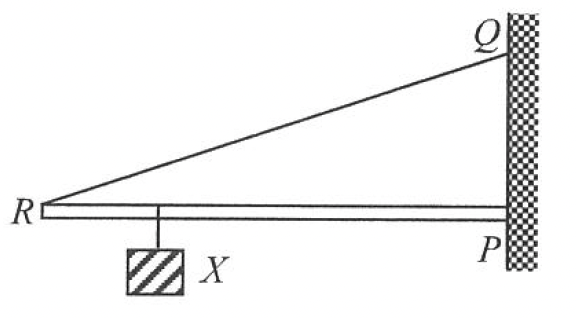
\includegraphics[width=0.33\textwidth]{assets/84e42251.png}
\par}
\begin{tasks}
    \task \qty{1.42}{N.m}
    \task \qty{1.05}{N.m}
    \task \qty{0.75}{N.m}
    \task \qty{0.70}{N.m}
\end{tasks}
}{A}

\newprob{1715332165}
{
一個勻質硬竿AB,以A為支軸,它由一金屬線接連牆壁上位於A點豎直上方的C點,使竿維持水平。竿上掛着負荷W。若將W逐漸從A移向B,下列哪些數量會增加?
{\par\centering
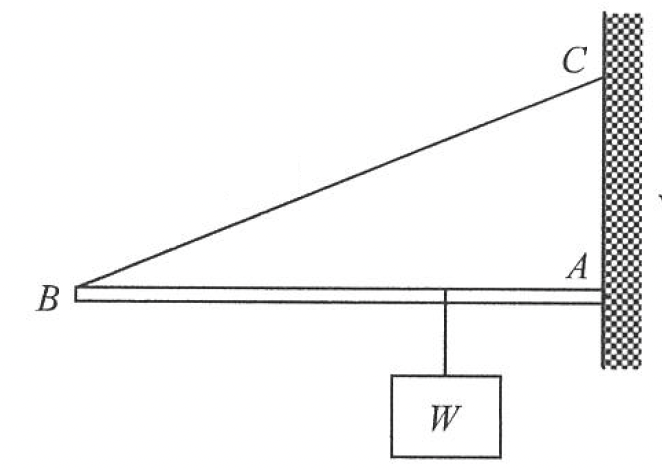
\includegraphics[width=.3\textwidth]{assets/a9b14a8d.png}
\par}
\begin{statements}
    \task 金屬線上的張力。
    \task 竿所受到的水平壓縮力。
    \task A點上的作用力的垂直分量。
\end{statements}
\begin{tasks}
    \task 只有(1)
    \task 只有(3)
    \task 只有(1)和(2)
    \task 只有(2)和(3)
\end{tasks}
}{C}

\newprob{1715331830}
{
一輕剛棒 $PO$ 的一端順滑地鉸接在牆上,另一端則以不能拉伸 的線接於$P$ 點正上方的$R$點。一負荷 $W$ 懸掛在棒上某點。若 棒保持水平,下列哪些改變會令線的張力增加?
{\par\centering
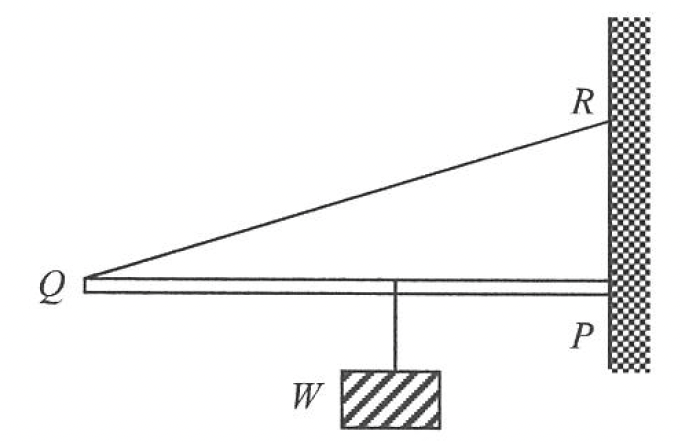
\includegraphics[width=.3\textwidth]{assets/4f96447b.png}
\par}
\begin{statements}
    \task
    將重量移向 $Q$
    \task
    更換較短的線,並分別接於 $PQ$ 和 $PR$ 的中點
    \task
    更換較長的線,並接於較 $R$ 爲高的一點
\end{statements}
\begin{tasks}
    \task 只有(1)
    \task 只有(2)
    \task 只有(3)
    \task 只有(1)和(2)
    \task 只有(1)和(3)
    \task 只有(2)和(3)
    \task (1), (2) 和 (3)
\end{tasks}
}{}

